\chapter{Biomass functions and nutrient contents of European beech, oak, sycamore maple and ash and their meaning for the biomass supply chain}
\label{chap:bm}
{\large Kai Husmann$^1$ - Sabine Rumpf$^2$ - J�rgen Nagel$^2$}\\

\vspace{3cm}
\noindent
$^1$Department of Forest Economics and Forest Management,\\ University of G�ttingen, B�sgenweg 3, 37077 G�ttingen, Germany \\

%\vspace{0.5cm}
\noindent
$^2$Northwest German Forest Research Institute,\\ Gr�tzelstra�e 2, 37079 G�ttingen, Germany\\

\vspace{\fill}
\noindent
Published in:\\
Journal of Cleaner Production.\\(DOI: X)


\cleardoublepage
%%%%%%%%%%%%%%
%% Abstract %%
%%%%%%%%%%%%%%
\section*{Abstract}
\label{chap:bm:Abstract}
Woody biomass from forests has great potential to provide a continuous and largely carbon-neutral raw material supply for the bio-based industry. As the demand for forestry products is already very high and steadily increasing, the question arises how to match the limited available wood resources to the growing demand for raw materials. Thus, there is an initial need to properly estimate the available biomass from forests. The success of a bio-based industry depends on an accurate forecast of the raw material flow coming from the forests for the entire biomass supply chain up to the industrial processing stage. Using easily measured input data, e. g. the tree diameter at breast height, biomass functions allow for a reliable prediction of tree species- and tree fraction-specific single-tree biomasses. In combination with nutrient content data, the site specific ecologically sustainable level of forestry use can be assessed and the site-specific wood utilisation potential can be fully exploited.
Biomass functions for the main tree species can be found in the literature. For other tree species, like sycamore or ash, however, there are only very specific studies available. As the wood potential of especially those species is recently often unused, goal of this study is to develop biomass functions and nutrient contents for European beech, oak, ash and sycamore for the fractions stem wood, bark, branches, and twigs.\\

For this purpose 139 trees were destructively sampled. Their single tree biomasses and nutrient contents were examined. This data was then used in a regression analysis to build generalised tree species- and tree fraction-specific biomass functions and nutrient contents for northern and central Germany.
We showed that the sycamore and ash biomass functions differed significantly from those of European beech and oak. Using oak biomass functions for the biomass estimation of sycamore and ash, as it is practised today, leads to a massive overestimation of the standing biomass in a test site up to 11 \% (21 tons / ha respectively).\\

The share of species-rich broadleaf forest stands, and thereby the importance of tree specific biomass functions, is increasing. The introduced models can help to exploit the huge biomass potential of those deciduous stands.\\

\subsection*{Keywords}
Biomass function - Nutrient content - Long-living tree species - Biomass supply chain - Site sustainability

\subsection*{Highlights}
\begin{itemize}
\item The effectivity of the biomass supply chain depends on reliable biomass estimation.
\item The wood potential of long-living tree species is recently often unused.
\item Biomass models for sycamore maple and ash can help gathering this potential.
\end{itemize}
%%%%%%%%%%%%%%%%%%
%% Introduction %%
%%%%%%%%%%%%%%%%%%
\section{Introduction}
\label{sec:bm:Introduction}

Biomass from forests has real potential to provide a continuous and largely carbon-neutral supply of material to the bio-based industry sector and can therefore make a significant contribution to a clean bio-based industry. Especially small dimensioned wood has huge potential for use in bio-refineries. \citet{ekman_2013} showed in Sweden that previously unused scrap wood can be used for the extraction of high quality chemical substances, such as bio-oils or antioxidants for use in the food or cosmetics industries. Supply of biomass from forestry can drive the economic growth of the entire bio-based chemical industry and make it competitive in the long-term, especially if wood fractions that have up to now been used as fuel wood are included. Innovative industries, such as the nanofiber or biochemistry industries, are increasing the demands on the forestry product-pool. The forest-based bio-economy is already an integral part of the global forestry sector \citep{hurmekoski_2013}. The European bio-based industry is currently a growing sector, with Germany playing a leading role \citep{hennig_2016}.

The global forestry industry is currently undergoing a process of change. The use of wood as raw materials in Germany has increased considerably in the last decades \citet{mantau_2012}. Changes in government energy policy and the development of new technology led to development of new markets, in particular for small dimensioned wood \citep{geldermann_2016, mccormick_2013}. The demand for forestry products is steadily rising, increasing the competition for raw timber. The question then is how to match the available wood resource to the demand for raw materials.

Just as it is for classical forestry \citep{mohring_1997}, knowledge of the available potential biomass is the main prerequisite for a functioning bio-based industry \citep{hennig_2016}. Using wood means that the nutrients bound in the wood are removed from the forest ecosystem. The biomass potential of a forest can only be utilised to an extent that, in the long-term, won�t deplete the supply of plant available nutrients in the forest ecosystem. In order to be able to exploit the woody biomass potential for the bio-based industry, the limit of the utilisation extend from the forests stands must be known \citep{block_2013, pretzsch_2014}. Therefore, reliable estimates of the quantity of biomass to be harvested, as well as reliable estimates of the amount of nutrients contained in these biomasses are required.

Using easily measured input data, such as diameter at breast height (dbh) or tree height, biomass functions enable the prediction of single-tree biomasses. Tree species and tree-fraction specific estimations of the forest biomass supply can be made. Using these biomass functions coupled with nutrient content data, the nutrient export can be estimated. In this way an ecologically sustainable level of forestry use can be calculated and the site specific wood utilization potential can be fully exploited.

The success of the bio-based industry depends to a great extent on the ability to accurately forecast the flow of raw materials in the integrated biomass supply chain \citep{geldermann_2016, how_2016}. Using biomass functions the relevant information for strategic operational decision-making can be generated for the entire biomass supply chain - from the forest stand to the industrial processing stage. Detailed biomass calculations can improve planning certainty along the entire value chain because the masses to be transported and those due at the factory gate can be forecasted very accurately. Biomass functions can therefore make an important contribution to increasing the planning capability, and thereby to cost reductions, in operative planning for forestry enterprises, wood logistics and wood industry firms.

Wood industry cluster studies on the availability of raw materials and on the market situation of the wood industry are the bases for the strategic orientation of the bio-economy industries \citep{mccormick_2013}. By using supply analyses and material flow simulations together with biomass functions decision support models can be parameterised which enable, for example, the computing of a continuous biomass supply chain \citep[e. g.][]{ruther_2007, wordehoff_2011, mantau_2012}.

Responsible biomass usage from forests has, next to its economic relevance, also very important social impacts. In 2006, under the terms of the Kyoto protocol, reporting of the carbon sequestration performance of forests became mandatory in Germany. The use of biomass functions is an integral part of this reporting process \citep{vallet_2006, tabacchi_2011, wordehoff_2011}.

In the literature there are numerous biomass functions \citep[e. g.][]{grote_2003, cienciala_2005, pretzsch_2014} and nutrient content figures \citep[e. g.][]{augusto_2000, jacobsen_2003, weis_2012, pretzsch_2014} available for the tree species European beech (Fagus sylvatica [L.]), common oak (Quercus robur [L.]) and sessile oak (Quercus petraea [L.]). For sycamore maple (Acer pseudoplatanus [L.]) and ash (Fraxinus excelsior [L.]) however, there are only few functions available. All literature functions found either do not cover the entire relevant diameter spectrum \citep[e. g.][]{albert_2014, alberti_2005} or do not allow fraction specific biomass estimation \citep{bunce_1968}.

The wood increment of long-term deciduous trees, which is the species group sycamore and ash belong to, was only used by 38 \% between 2002 and 2012 \citep{ti_2014}. This is certainly partially reasoned by the fact that reliable planning methods for long-term deciduous species are not available. The question then arises if the predictions of the woody biomass in these stands could be improved by using specific biomass functions and nutrient contents for sycamore and ash. Specific biomass functions for these species could help making the recently unused potential available for the bio-based industry.

The goal of this study is to develop biomass functions for European beech, oak, sycamore and ash by means of regression analysis, using data gathered in northern and central Germany. Functions are developed for the tree fractions stem wood (diameter > 7cm without bark), bark of stem wood, branches (1 - 7cm with bark), and twigs (< 1cm with bark). The differences in these biomass functions are examined at single-tree and stand level by means of a sensitivity analysis in an exemplary test stand. The nutrient content in the different tree fractions of the tree species studied are determined and used as the basis for quantifying the nutrient removal by harvesting. The amount of nutrients that are removed from the forest ecosystem is then determined by multiplying the nutrient content with the biomass.

%%%%%%%%%%%%%%%%%%%%%%%%%%%
%% Materials and Methods %%
%%%%%%%%%%%%%%%%%%%%%%%%%%%
\section{Materials and Methods}
\label{sec:bm:methods}
With the goal of quantifying biomass and nutrient content 139 vital trees were studied (Table 1). The sample plots for beech and oak represented as many different growing areas and site conditions as possible. The high nutrient requirements of sycamore and ash meant that the sample plots for these species were exclusively on nutrient-rich, calcareous substrates. Per plot 2 - 4 trees were chosen (Fig. \ref{fig:bm:fig1}). Both within each sample site, and across the plots as a whole, the aim was to collect trees from a wide and evenly distributed diameter range.

\begin{figure}
	\center
	\includegraphics[width=0.75\textwidth]{Grafiken/bm/Fig_1_Locations.eps}
	\caption{Locations of the 54 sampled plots. Source of the background map: \citet{facg_2014}.}
	\label{fig:bm:fig1}
\end{figure}


%% TAB 1

%%-------------------------------------%%
%% Data sampling and sample processing %%
%%-------------------------------------%%
\subsection{Data sampling and sample processing}
\label{subsec:bm:methods:sampling}

Dbh, height at crown base and tree height were measured for each tree. The fraction volumes of the trees were determined using randomized branch sampling (RBS). RBS is an efficient and bias free sampling method for estimating tree fractions \citep{saborowski_1999, Gregoire_2008}. Since this method was firstly described \citet{jessen_1955} it has been used in other studies, including those from \citet{valentine_1984}, \citet{gaffrey_1999} and \citet{affleck_2015}. This multi-stage sampling method assumes proportionality between the target quantity and an easily measurable proxy. Because an allometric relationship exists between branch volume and branch base diameter \citep{west_1999}, the RBS method makes it possible to estimate the wood volume by measuring only a subset of branch lengths and branch diameters in the tree crowns. The stem form was assessed by section-wise diameter measurements at certain tree heights up to the crown base. In order to determine the specific bulk density and nutrient contents, up to 12 samples, covering all diameters of the tree, were collected per tree using the Importance Sampling \citep{Gregoire_2008}.


%%-------------------%%
%% Biomass functions %%
%%-------------------%%
\subsection{Biomass functions}
\label{subsec:bm:methods:bm_functions}

Biomass functions.

%%----------------------%%
%% Sensitivity analysis %%
%%----------------------%%
\subsection{Sensitivity analysis}
\label{subsec:bm:methods:sensitivity}

Sensitivity.

%%-------------------%%
%% Nutrient contents %%
%%-------------------%%
\subsection{Nutrient contents}
\label{subsec:bm:methods:nutrients}

Sensitivity.

%%%%%%%%%%%%%
%% Results %%
%%%%%%%%%%%%%
\section{Results}
\label{sec:bm:results}

%%-------------------%%
%% Biomass functions %%
%%-------------------%%
\subsection{Biomass functions}
\label{subsec:bm:results:bm_functions}

Biomass functions.


%%----------------------%%
%% Sensitivity analysis %%
%%----------------------%%
\subsection{Sensitivity analysis}
\label{subsec:bm:results:sensitivity}

Sensitivity.

%%-------------------%%
%% Nutrient contents %%
%%-------------------%%
\subsection{Nutrient contents}
\label{subsec:bm:results:nutrients}

Nutrient.

%%%%%%%%%%%%%%%%
%% Discussion %%
%%%%%%%%%%%%%%%%
\section{Discussion}
\label{sec:bm:discussion}

%%-------------------%%
%% Biomass functions %%
%%-------------------%%
\subsection{Biomass functions}
\label{subsec:bm:discussion:bm_functions}

Biomass functions.

%%----------------------%%
%% Sensitivity analysis %%
%%----------------------%%
\subsection{Sensitivity analysis}
\label{subsec:bm:discussion:sensitivity}

Sensitivity.

%%-------------------%%
%% Nutrient contents %%
%%-------------------%%
\subsection{Nutrient contents}
\label{subsec:bm:discussion:nutrients}

Nutrients.

%%%%%%%%%%%%%%%%%
%% Conclusions %%
%%%%%%%%%%%%%%%%%
\section{Conclusions}
\label{sec:bm:conclusions}

Conclusion

%%%%%%%%%%%%%%%%%%%%%%
%% Acknowledgements %%
%%%%%%%%%%%%%%%%%%%%%%
\section*{Acknowledgements}
\label{sec:bm:acknowledgements}
We would like to thank the German Science Foundation (DFG) for financial support of this study (Sachbeihilfe SA 415/5-1) and Dr. B�ckmann of the Lower Saxony Forest Planning Office for his kind provision of the inventory data.
Moreover, we would like to thank two anonymous reviewers for their helpful comments.
